\documentclass[11pt]{article}

\usepackage[T1]{fontenc}
\usepackage[utf8]{inputenc}
\usepackage[a4paper,margin=2.5cm]{geometry}
\usepackage{amsmath}
\usepackage{newtxtext,newtxmath}
\usepackage{microtype}
\usepackage{xcolor}
\usepackage{enumitem}
\usepackage{graphicx}
\usepackage{float}
\usepackage[percent]{overpic}
\usepackage{hyperref}

\definecolor{responseblue}{HTML}{1F4E79}
\definecolor{commentgray}{HTML}{4D4D4D}
\definecolor{rulegray}{HTML}{C8CDD2}

\hypersetup{
  colorlinks=true,
  linkcolor=responseblue,
  urlcolor=responseblue,
  citecolor=responseblue,
  pdftitle={Response to Referee Reports -- ER12738}
}

\setlength{\parindent}{0pt}
\setlength{\parskip}{0.65em}
\setlist[enumerate]{leftmargin=*,itemsep=0.45em,topsep=0.25em}
\raggedbottom

\newenvironment{refereecomment}
  {%
    \par
    \begingroup
    \color{commentgray}
    \itshape
    \setlength{\leftskip}{1.4em}
    \setlength{\rightskip}{1.4em}
  }
  {%
    \par
    \endgroup
  }

\newcommand{\refereelabel}{%
  \par\smallskip
  {\color{commentgray}\bfseries Referee Comment}\par
}

\newcommand{\responselabel}{%
  \par\medskip
  {\color{responseblue}\bfseries Author Response}\par
}

\newcommand{\pointseparator}{%
  \par\bigskip
  {\color{rulegray}\hrule}
  \par\bigskip
}

\title{\textbf{Response to Referee Reports}\\[0.35em]
  \large Manuscript ER12738}
\author{}
\date{}

\begin{document}

\begin{flushleft}
\textbf{Re: ER12738}\\
\textit{Scaling behaviors in simulated collagen fibrils}\\
by Robert Bertoldo Tavares, Michael Ferreira de Souza, Béla Suki And Ascânio D. Araújo

\medskip

Dear,

Ph.D. Margaret Foster\\
Senior Assistant Editor\\
Physical Review E

\medskip

Thank you for obtaining a Referee report on our manuscript by Robert Bertolo et al. (ER12738).
We would like to submit a new version of our manuscript ER12738, as we feel that we can answer, in an appropriate way, the questions and comments addressed in the reports of the Referees. We would be very pleased if you could give further consideration to our submission.
\end{flushleft}

\bigskip

\maketitle
\vspace{-2.5em}

\section*{\LARGE Response to Referee 1}

\subsection*{Point 1 (R1-1): Physical grounding of the surface-diffusion parameter \(T_s\)}

\refereelabel
\begin{refereecomment}
\(T_s\) controls the number of post-attachment lateral diffusion steps and
therefore governs the ratio between the molecular relaxation timescale and the
fibril growth rate. In real type I collagen fibrillogenesis, this ratio is
modulated by temperature, collagen concentration, pH, and ionic strength, all
experimentally accessible quantities. The authors acknowledge that \(T_s\) has
no direct mapping to biochemical conditions (e.g., pH), yet proceed to
speculate in the concluding paragraph about evolutionary fine-tuning of fibril
compactness and its role in diseases such as pulmonary emphysema and aortic
aneurysm. These biological inferences are unsupported without at least a
qualitative discussion of how \(T_s\) relates to measurable physical or
physiological variables. The manuscript would be strengthened considerably by
such a discussion, even at the order-of-magnitude level.
\end{refereecomment}

\responselabel
We thank the Referee for the opportunity to clarify the physical basis
of the parameter \(T_s\). Experiments show that physicochemical conditions—such as temperature, pH, ionic strength, and concentration—alter electrostatic interactions and growth kinetics, simultaneously affecting incorporation and relaxation. The parameter $T_s$ captures the net effect of assembly conditions on local rearrangement during growth. However, calibrating it against specific experimental variables would require independent estimates of incorporation and relaxation timescales, which is beyond the scope of this work.

We have revised the model description to make this interpretation explicit.
We also removed the evolutionary and disease-specific
extrapolations from the conclusion, which is now limited to the model result
that greater effective post-attachment relaxation produces more compact
fibrils and greater resistance to failure in the simulations.

The following paragraph has been added to the revised manuscript:

\textit{The formation of real fibrils is driven by electrostatic forces \cite{Parkinson1995} that favor lateral association and minimize exposed surface area \cite{Kadler1987,Parkinson1995}.
During collagen fibrillogenesis, the resulting molecular organization reflects the competition between the rate of molecular incorporation and the opportunity for local rearrangement during growth.
Experimental studies show that physicochemical conditions—such as temperature, collagen concentration, pH, ionic strength, and buffer composition—modify electrostatic interactions, lateral association, and assembly kinetics \cite{Kadler1988,Yang2009,Gobeaux2008,Kalbitzer2018,Morozova2018}, simultaneously altering incorporation and relaxation rates to shift this balance. Following \cite{Parkinson1995}, this growth-to-relaxation balance is represented in a discrete, coarse-grained form through a dimensionless surface diffusion parameter $T_s$, where increasing $T_s$ provides greater opportunity for post-attachment relaxation relative to continued growth and leads to progressively more compact fibrils.}

\pointseparator

\subsection*{Point 2 (R1-2): Attribution of Self-Organized Criticality}

\refereelabel
\begin{refereecomment}
The authors claim that the rupture process exhibits SOC on the basis that the
avalanche size distribution follows a power law. This reasoning is
insufficient. SOC requires that a system spontaneously evolves toward a
critical state without external tuning of a control parameter, the canonical
example being the Bak--Tang--Wiesenfeld sandpile. In the present model, the
external force \(F\) is continuously increased by the experimenter until
failure occurs. The system is driven, not self-organizing.

Critically, two of the papers the authors themselves cite to support the SOC
claim (refs. [42] and [43], Zapperi et al., PRL 1997 and PRE 1999) make no
reference to SOC. Instead, Zapperi et al. explicitly characterize the breakdown
point as a first-order transition and draw an analogy with spinodal nucleation,
a fundamentally different phenomenology. The correct terminology for the
dynamics observed here is ``avalanche statistics in driven disordered
fracture,'' not SOC.

Furthermore, the power-law regime in Fig.~9(a) spans at most two orders of
magnitude in avalanche size, a marginal range. No statistical validation of
the power-law hypothesis is presented (e.g., maximum likelihood estimation of
the exponent, Kolmogorov--Smirnov test, or comparison with alternative
distributions following the methodology of Clauset et al., SIAM Review 51,
661, 2009). The claim of scale-free behavior therefore rests on insufficiently
rigorous grounds.
\end{refereecomment}

\responselabel
We thank the Referee for this important correction. We agree that an
approximately linear regime in a binned log--log plot is insufficient to
establish Self-Organized Criticality. Because the external force is increased
stepwise, damage is irreversible, and failed molecules do not recover, we have
removed the SOC interpretation and instead describe the process as avalanche
dynamics in a driven disordered fracture system.

Following the Referee's statistical and operational suggestions, we
reanalyzed the raw, integer-valued sizes of preterminal avalanches. At
each fixed force \(F\), an avalanche comprises all
molecules removed during the successive damage sweeps performed before the
next force increment. Here, an avalanche denotes the complete damage response
at one force step and does not imply spatial connectivity or system-spanning
failure. The terminal event that eliminates the continuous
load-bearing path and causes complete rupture is excluded. The revised data
set contains 67,026,212 preterminal events across the ten values of \(T_s\).
We then evaluated whether the upper tail of the avalanche-size distribution
could be described by a power law with an exponential cutoff. For compact
presentation, we write this model in scaling form as

\[
p(s)\sim s^{-\gamma}\exp(-s/s_c),
\qquad s\geq s_{\min}.
\]

This form is widely used for algebraic tails limited by a finite
characteristic scale, including avalanche and fracture processes
(\href{https://doi.org/10.1103/PhysRevE.59.5049}{Zapperi et al., 1999};
\href{https://doi.org/10.1137/070710111}{Clauset, Shalizi, and Newman, 2009};
\href{https://doi.org/10.1371/journal.pone.0019779}{Klaus, Yu, and Plenz,
2011}).
The exponent \(\gamma\) characterizes the algebraic sector, while \(s_c\)
characterizes the cutoff scale, which may reflect finite-size and
model-specific constraints. The scaling expression is used here for
readability; numerical estimation and KS calculations use the fully normalized
discrete model.

We estimated \(\gamma\) and \(s_c\) by exact discrete maximum likelihood without
binning. For each \(T_s\), the lower threshold \(s_{\min}\) was selected
objectively by minimizing the discrete Kolmogorov--Smirnov distance after
fitting the model parameters, following the procedure of
\href{https://doi.org/10.1137/070710111}{Clauset, Shalizi, and Newman (2009)}
for identifying the onset of a tail regime. Alternative selection criteria and
limitations of this procedure are discussed by
\href{https://arxiv.org/abs/1209.1270}{Corral, Deluca, and Ferrer-i-Cancho
(2012)}. Thus, neither the fitted interval nor the exponent was selected by
visual inspection.

In the compact-fibril regime, \(T_s\geq512\), the independently selected
thresholds are tightly grouped, \(18\leq s_{\min}\leq21\), and each fit
contains between 354,967 and 465,153 tail events. The observed KS distances
are only \(8.5\times10^{-4}\) to \(1.4\times10^{-3}\). At the same time, both
tail parameters stabilize:

\[
\gamma=2.204\pm0.034,
\qquad
s_c=101.0\pm5.6,
\]

where the quoted dispersions describe variation among the four compact-regime
conditions. The simultaneous stability of \(s_{\min}\), \(\gamma\), and \(s_c\),
together with the very small KS discrepancy and the large number of fitted
events, provides the central evidence for a common cutoff-power-law tail in
the compact regime. Events below \(s_{\min}\) remain visible in the revised
figure but are not assumed to follow the same tail model, which is precisely
the role of a statistically selected lower threshold. The complete
distributions and the evolution of the fitted parameters are shown in
Figs.~\ref{fig:avalanche-distributions} and
\ref{fig:avalanche-parameters}, respectively.

\begin{figure}[!htbp]
  \centering
  \begin{overpic}[width=0.98\textwidth]{figure_1.png}
    \put(4,23.4){\color{white}\rule{16\unitlength}{2.5\unitlength}}
    \put(24,23.4){\color{white}\rule{16\unitlength}{2.5\unitlength}}
    \put(44,23.4){\color{white}\rule{16\unitlength}{2.5\unitlength}}
    \put(64,23.4){\color{white}\rule{16\unitlength}{2.5\unitlength}}
    \put(84,23.4){\color{white}\rule{16\unitlength}{2.5\unitlength}}
    \put(4,0.1){\color{white}\rule{16\unitlength}{2.4\unitlength}}
    \put(24,0.1){\color{white}\rule{16\unitlength}{2.4\unitlength}}
    \put(44,0.1){\color{white}\rule{16\unitlength}{2.4\unitlength}}
    \put(64,0.1){\color{white}\rule{16\unitlength}{2.4\unitlength}}
    \put(84,0.1){\color{white}\rule{16\unitlength}{2.4\unitlength}}
    \put(12,24.6){\makebox(0,0){\fontsize{5}{5}\selectfont Avalanche size, \(s\)}}
    \put(32,24.6){\makebox(0,0){\fontsize{5}{5}\selectfont Avalanche size, \(s\)}}
    \put(52,24.6){\makebox(0,0){\fontsize{5}{5}\selectfont Avalanche size, \(s\)}}
    \put(72,24.6){\makebox(0,0){\fontsize{5}{5}\selectfont Avalanche size, \(s\)}}
    \put(92,24.6){\makebox(0,0){\fontsize{5}{5}\selectfont Avalanche size, \(s\)}}
    \put(12,1.2){\makebox(0,0){\fontsize{5}{5}\selectfont Avalanche size, \(s\)}}
    \put(32,1.2){\makebox(0,0){\fontsize{5}{5}\selectfont Avalanche size, \(s\)}}
    \put(52,1.2){\makebox(0,0){\fontsize{5}{5}\selectfont Avalanche size, \(s\)}}
    \put(72,1.2){\makebox(0,0){\fontsize{5}{5}\selectfont Avalanche size, \(s\)}}
    \put(92,1.2){\makebox(0,0){\fontsize{5}{5}\selectfont Avalanche size, \(s\)}}
  \end{overpic}
  \caption{Complete distributions of preterminal avalanche sizes
  (open circles) and the extended exponentially cutoff power-law
  tails (red lines) for the ten values of \(T_s\). The parameters displayed in
  each panel were estimated by maximum likelihood using only events with
  \(s\geq s_{\min}\); the continuation below \(s_{\min}\) is shown only to
  place the fitted tail in the context of the complete empirical
  distribution.}
  \label{fig:avalanche-distributions}
\end{figure}

\begin{figure}[!htbp]
  \centering
  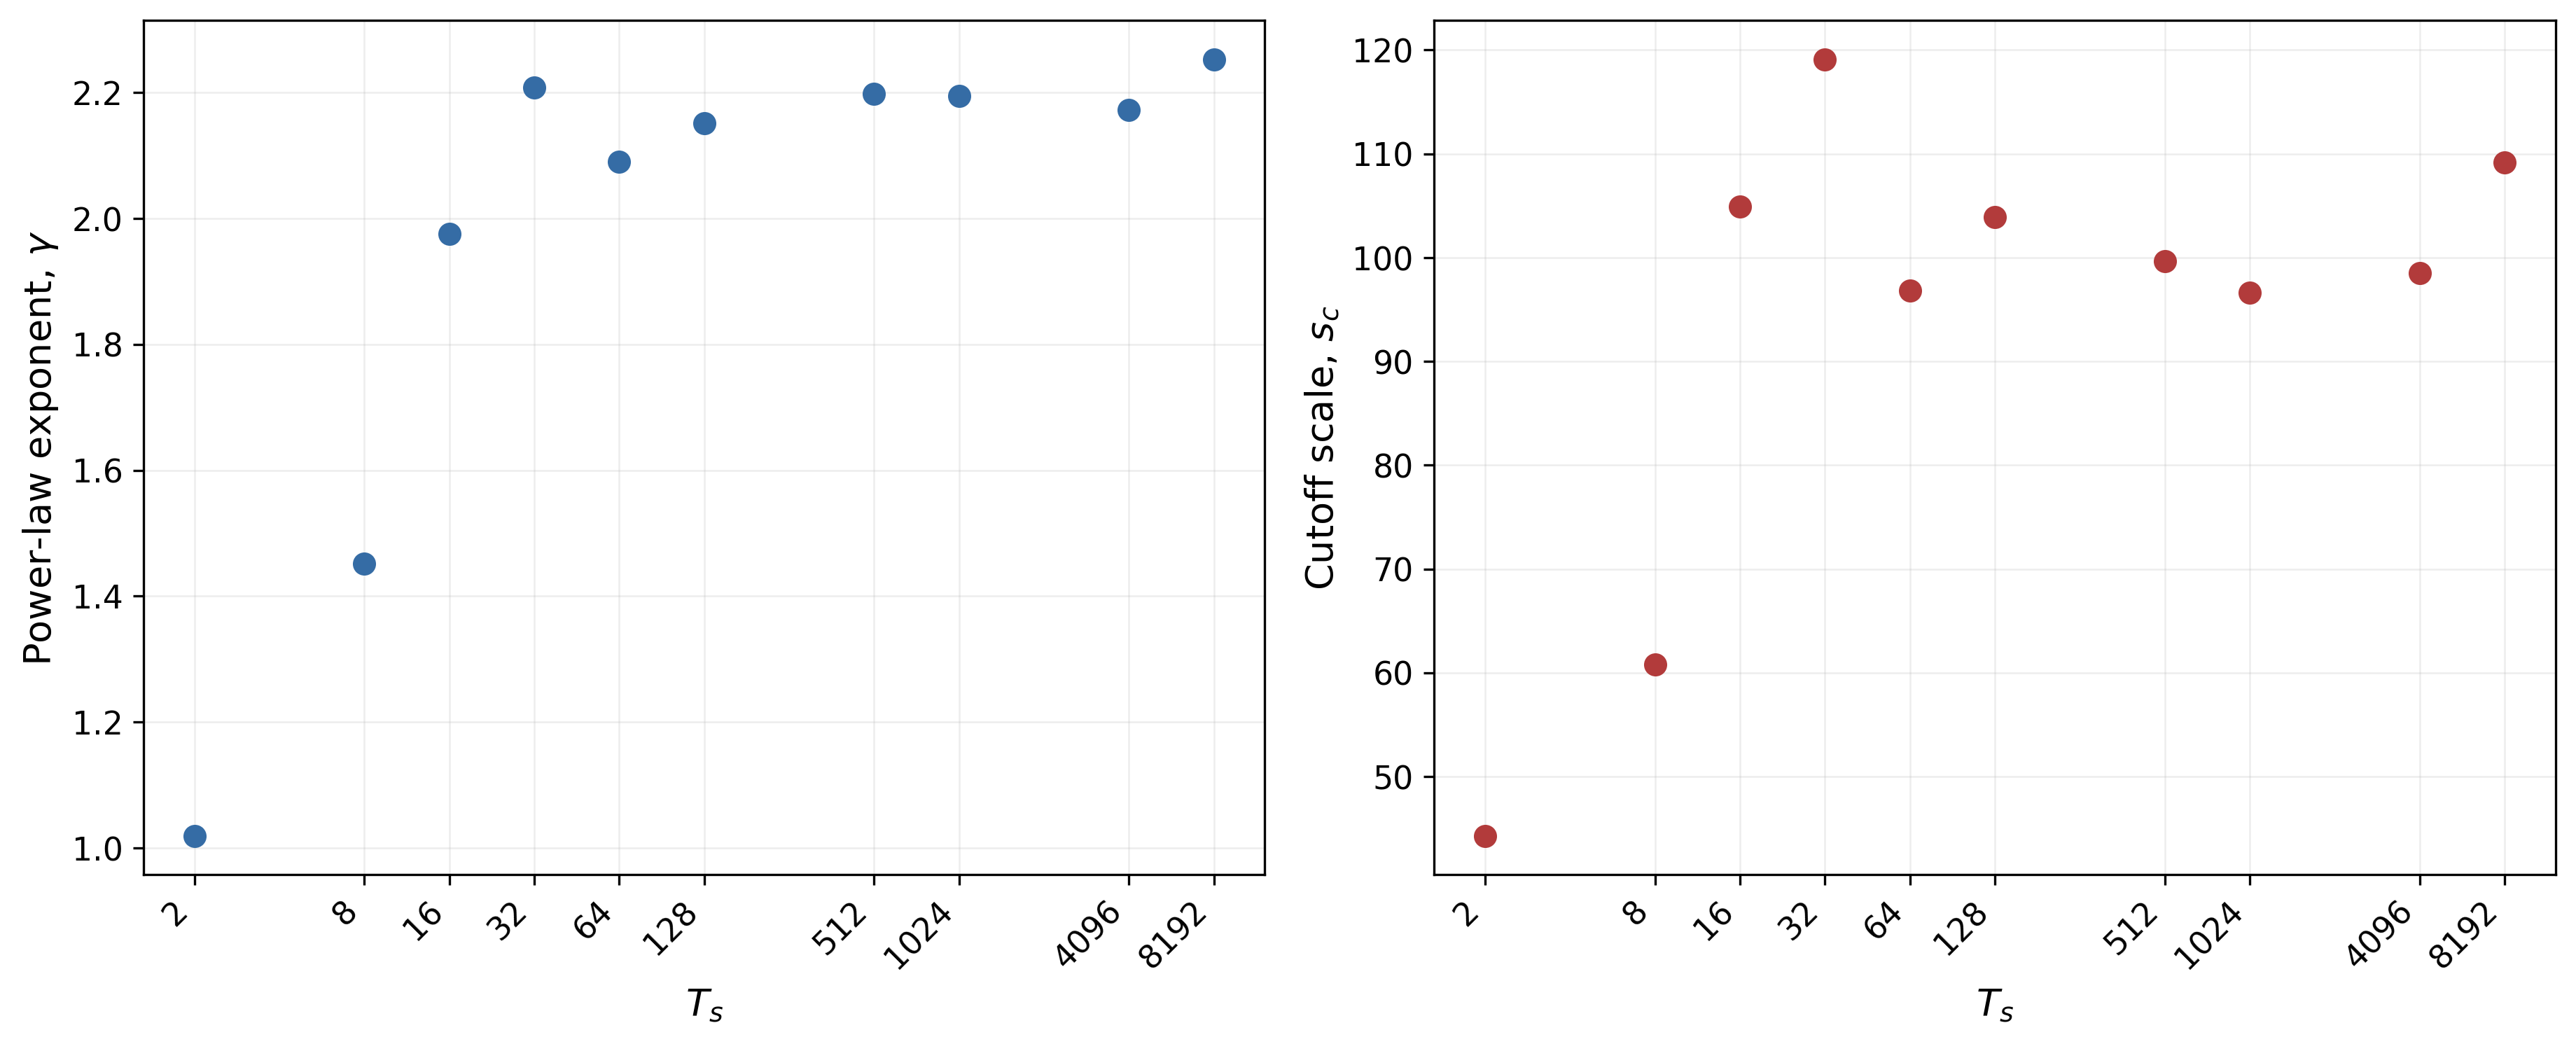
\includegraphics[width=0.98\textwidth]
    {figure_2.png}
  \caption{Evolution of the maximum-likelihood tail parameters with the
  dimensionless surface-relaxation parameter \(T_s\): (a) power-law exponent
  \(\gamma\) and (b) exponential
  cutoff scale \(s_c\). For \(T_s\geq512\), both quantities stabilize around
  \(\gamma=2.204\pm0.034\) and \(s_c=101.0\pm5.6\), where the quoted dispersions
  describe variation among the four compact-regime conditions.}
  \label{fig:avalanche-parameters}
\end{figure}

The synthetic goodness-of-fit calculation tests the stronger null hypothesis
that the observations are generated exactly by the fitted parametric family.
With very large samples, small finite-size and scaling corrections can make
such deviations detectable even when maximum likelihood accurately recovers
the exponent and the tail form. This situation has direct precedents: it has
been reported for neuronal-avalanche data analyzed using maximum likelihood,
KS, finite-size scaling, and comparisons with alternatives
(\href{https://doi.org/10.1371/journal.pone.0019779}{Klaus, Yu, and Plenz,
2011}; \href{https://doi.org/10.1016/j.neuron.2018.10.045}{Ponce-Alvarez et
al., 2018}), and Deluca and Corral documented related limitations for
simulated power-law tails and truncated distributions
(\href{https://doi.org/10.2478/s11600-013-0154-9}{Deluca and Corral, 2013}).
We therefore report the synthetic test, but interpret it together with the
magnitude of the observed KS distance, parameter stability, same-support model
comparisons, and the finite-size control described below.

As an independent control, we applied the same maximum-likelihood analysis to
two-dimensional percolation exactly at the critical point. Following Stauffer
and Aharony (1994), the finite-size cluster distribution satisfies

\[
n_s(L)\sim s^{-\tau_{\mathrm{perc}}}f(s/s_c),
\qquad
\tau_{\mathrm{perc}}=\frac{187}{91}\simeq2.055.
\]

For \(L=1000\), 2000, 5000, and 10000, the fitted exponents were respectively
1.951, 1.985, 2.013, and 2.027. The estimate converges monotonically toward
the exact value and differs from it by only about 1.4\% for the largest
system, although the strict synthetic test rejects the ideal parametric form.
As shown in Fig.~\ref{fig:percolation-control}, the size-dependent cutoff moves
systematically toward larger clusters while the maximum-likelihood exponent
converges toward \(187/91\). This control demonstrates in a system with
independently known scaling that formal rejection of an exact distribution can
coexist with quantitatively accurate recovery of its algebraic exponent in the
presence of finite-size corrections. It is used as a methodological
validation, not to assign the fracture avalanches to the percolation
universality class.

\begin{figure}[H]
  \centering
  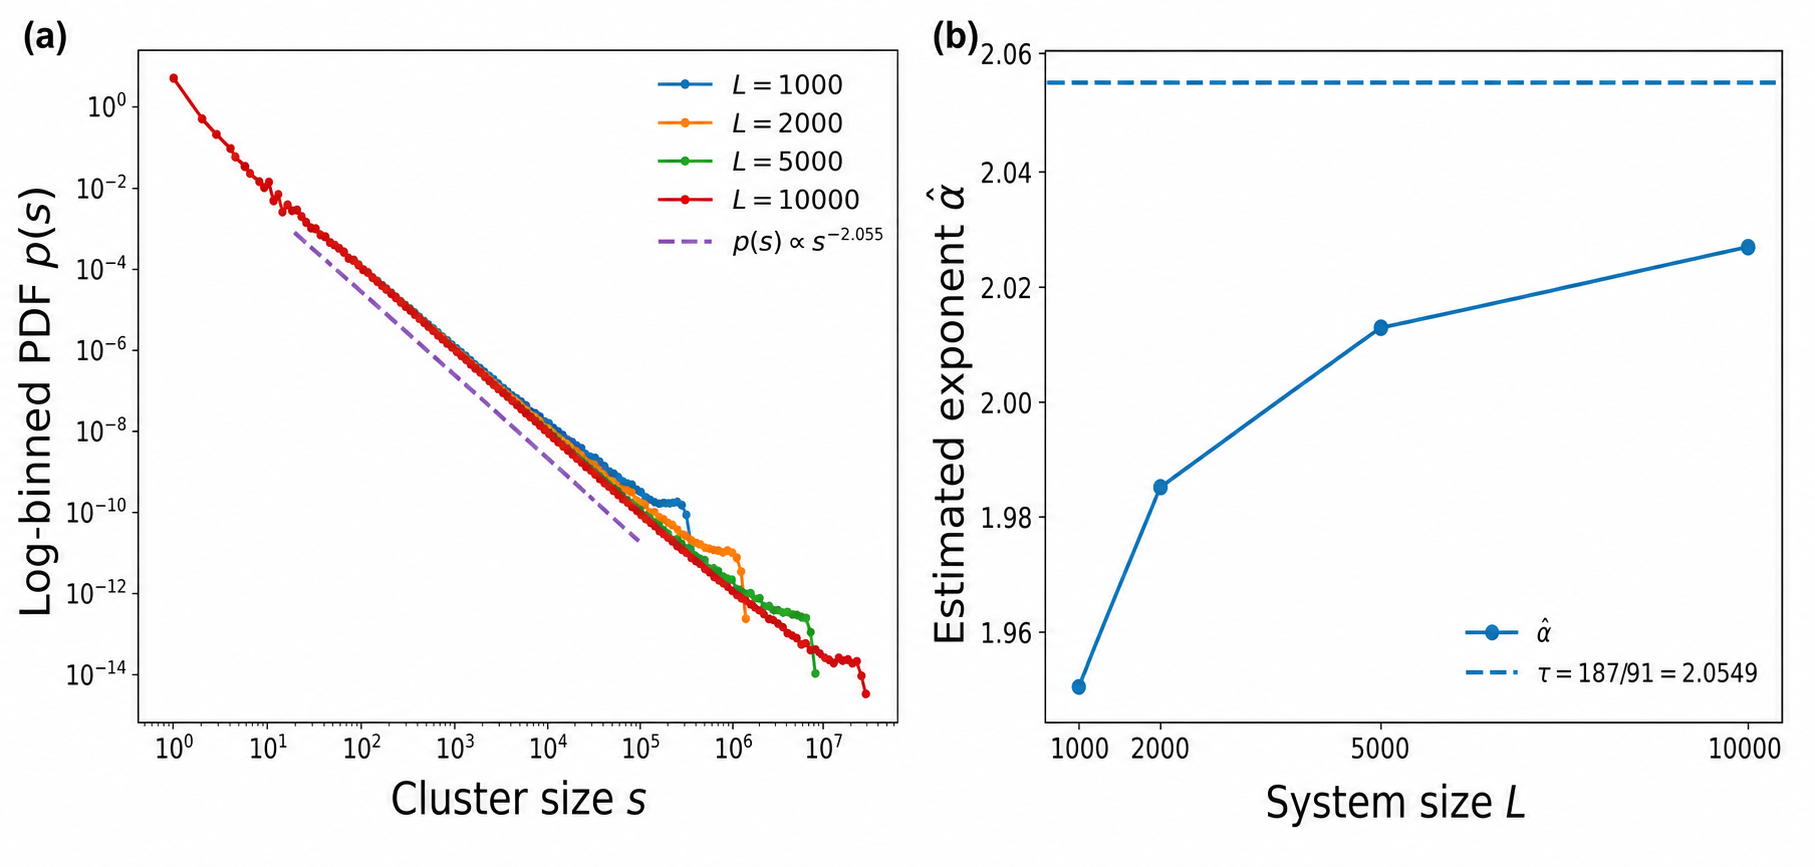
\includegraphics[width=0.96\textwidth]
    {figure_3.png}

  \caption{Validation of the maximum-likelihood exponent estimation using
  two-dimensional critical percolation. (a) Log-binned cluster-size
  distributions for different system sizes \(L\). The dashed line indicates
  the theoretical algebraic behavior \(p(s)\propto s^{-187/91}\). The
  finite-size cutoff moves toward progressively larger cluster sizes as \(L\)
  increases. (b) Maximum-likelihood estimate of the exponent as a function of
  \(L\). The dashed horizontal line indicates the exact value
  \(\tau=187/91\simeq2.0549\). The estimate approaches the theoretical value
  monotonically, reaching \(\widehat{\tau}=2.0273\) for \(L=10000\).}
  \label{fig:percolation-control}
\end{figure}

Our revised conclusion therefore does not rest on a straight line in a
log--log plot. It is supported by unbinned discrete data, an objectively
selected \(s_{\min}\), exact maximum likelihood, very small KS distances,
hundreds of thousands of tail events per compact condition, stable values of
\(\gamma\) and \(s_c\), and a finite-size control that recovers a known
theoretical exponent. We conclude that the preterminal avalanche-size
distributions possess an upper tail described by a power law with an
exponential cutoff; we do not describe the complete distribution as a pure or
strictly scale-free power law.

% TODO Issue #5: insert the finalized same-support likelihood comparison and
% block-bootstrap confidence intervals.

\clearpage
\pointseparator

\subsection*{Point 3 (R1-3): Interpretation of \(\gamma>5/2\) in fiber-bundle theory}

\refereelabel
\begin{refereecomment}
The authors interpret their measured exponent \(\gamma\approx2.8\) (at high
\(T_s\)) as evidence of a regime beyond equal load sharing (ELS), signaling a
crossover to global load-sharing universality. This interpretation is
incorrect.

In fiber-bundle models, \(\gamma=5/2\) is the exact mean-field result for ELS,
the limiting case of maximally global stress redistribution (Hemmer \& Hansen,
J. Appl. Mech. 59, 909, 1992; Daniels, Proc. R. Soc. London A 183, 405, 1945).
There is no established theoretical framework that predicts or interprets
exponents above \(5/2\) in this context.

Moreover, Pradhan, Hansen \& Chakrabarti (Rev. Mod. Phys. 82, 499, 2010), also
cited by the authors, demonstrate that within ELS, the avalanche exponent
undergoes a crossover from \(\gamma=5/2\) (generic regime, away from failure) to
\(\gamma=3/2\) (near the critical breakdown point). That is, as stress
redistribution becomes maximally global near rupture, the exponent DECREASES,
not increases. The authors' claim that \(\gamma>5/2\) signals increasingly
global load sharing is therefore the opposite of what the established theory
predicts.

The observed deviation from \(5/2\) is more plausibly attributable to
finite-size effects, limited ensemble statistics (10 fibrils per \(T_s\) value),
the restricted range over which the power law is fitted, or the specific
definition of avalanche adopted in the model. A sensitivity analysis with
respect to the Weibull modulus \(m\) (fixed at \(m=2\) throughout, following
Ref.~[35]) would also help assess the robustness of the exponents.
\end{refereecomment}

\responselabel
We thank the Referee and agree that the original comparison of the binned-fit
exponent with the equal-load-sharing value \(5/2\) was not justified. We have
removed the claim that an exponent above \(5/2\) signals increasingly global
load sharing or a new universality regime.

The revised analysis uses the preterminal force-step avalanche defined above and an
exponentially cutoff power law fitted by discrete maximum likelihood. In the
compact regime it yields the stable effective tail parameter
\(\gamma=2.204\pm0.034\) together with the finite cutoff scale
\(s_c=101.0\pm5.6\). Because \(\gamma\) is a parameter of a cutoff distribution
rather than the exponent of a pure asymptotic power law, we do not identify it
with the equal-load-sharing result or use it to classify the
stress-redistribution universality of the model.

The revised ensemble contains 50 fibril geometries for every \(T_s\), rather
than the ten geometries used in the original figure, with 1000 stochastic
rupture realizations for each geometry. All simulations considered here use
Weibull modulus \(m=2\). We therefore restrict the statistical conclusion to
this model choice and do not claim robustness with respect to \(m\).

\pointseparator

\subsection*{Point 4 (R1-4): Cross-sectional fractal dimension and three-dimensional mechanical structure}

\refereelabel
\begin{refereecomment}
The fractal dimension is measured in 2D but used to characterize a 3D
mechanical problem. \(D_f\) is estimated from 2D cross-sectional projections
(\(x\)-\(z\) plane), yet the backbone identification and the entire fracture
simulation are three-dimensional. The relationship between the 2D
cross-sectional \(D_f\) and the 3D structural properties that govern mechanical
response is not established. The authors use the 2D \(D_f\) as a proxy for
overall fibril compactness without justification. This connection should
either be derived or explicitly discussed as an assumption with its
limitations.
\end{refereecomment}

\responselabel
We thank the Referee for pointing out that the original manuscript did not
adequately establish the connection between the cross-sectional fractal
dimension and the three-dimensional mechanical structure. The cross-sectional
\(D_f\) characterizes transverse packing, which is directly relevant to the
rupture model because the tensile stress at each axial position is determined
by the load-bearing area \(N(i)\) of the corresponding cross-section, while
molecular resistance depends on coordination within the three-dimensional
backbone.

To test this connection explicitly, for each \(T_s\) we obtained \(D_f\) from
the ensemble mass--radius curve constructed using 11 transverse cross-sections
from each of 50 independent fibrils. From the corresponding three-dimensional
load-bearing backbones, we measured four mechanically relevant descriptors:
the mean cross-sectional load-bearing area \(\langle N\rangle\); the mean
molecular coordination \(\langle K\rangle\); the axial coefficient of
variation of the load-bearing area,
\[
  \mathrm{CV}(N)=
  \frac{1}{\langle N\rangle}
  \left[
    \frac{1}{S_y-1}
    \sum_{i=1}^{S_y}\left(N(i)-\langle N\rangle\right)^2
  \right]^{1/2},
\]
which quantifies the relative variation of \(N(i)\) along the 201 axial layers;
and the mean molecular stress exposure at unit force,
\(\langle\sigma_M\rangle_{F=1}\), obtained by evaluating the molecular stress
defined in Eq.~(3) at \(F=1\) and averaging it over the backbone molecules.
These descriptors were averaged over the independent fibrils, with their
uncertainties reported as standard errors of the mean. The uncertainty in
\(D_f\) corresponds to the standard error of the linear mass--radius fit.
Because the relationships are monotonic and approach plateaus rather than
remaining linear, associations were evaluated using Spearman's rank
correlation coefficient, \(\rho\)
(\href{https://doi.org/10.2307/1412159}{Spearman, 1904};
\href{https://doi.org/10.1213/ANE.0000000000002864}{Schober et al., 2018}),
between the ten \(T_s\)-averaged conditions.

The cross-sectional \(D_f\) was positively associated with the mean
load-bearing area (\(\rho=0.997\)) and mean molecular coordination
(\(\rho=0.997\)), and inversely associated with the axial variability of the
load-bearing area (\(\rho=-0.778\)) and mean molecular stress exposure at unit
force (\(\rho=-0.979\)). Thus, increasing \(D_f\) accompanies cross-sections
that contain more load-bearing material, greater molecular coordination,
reduced axial heterogeneity, and lower mean stress exposure for the same
applied force.

\begin{figure}[H]
  \centering
  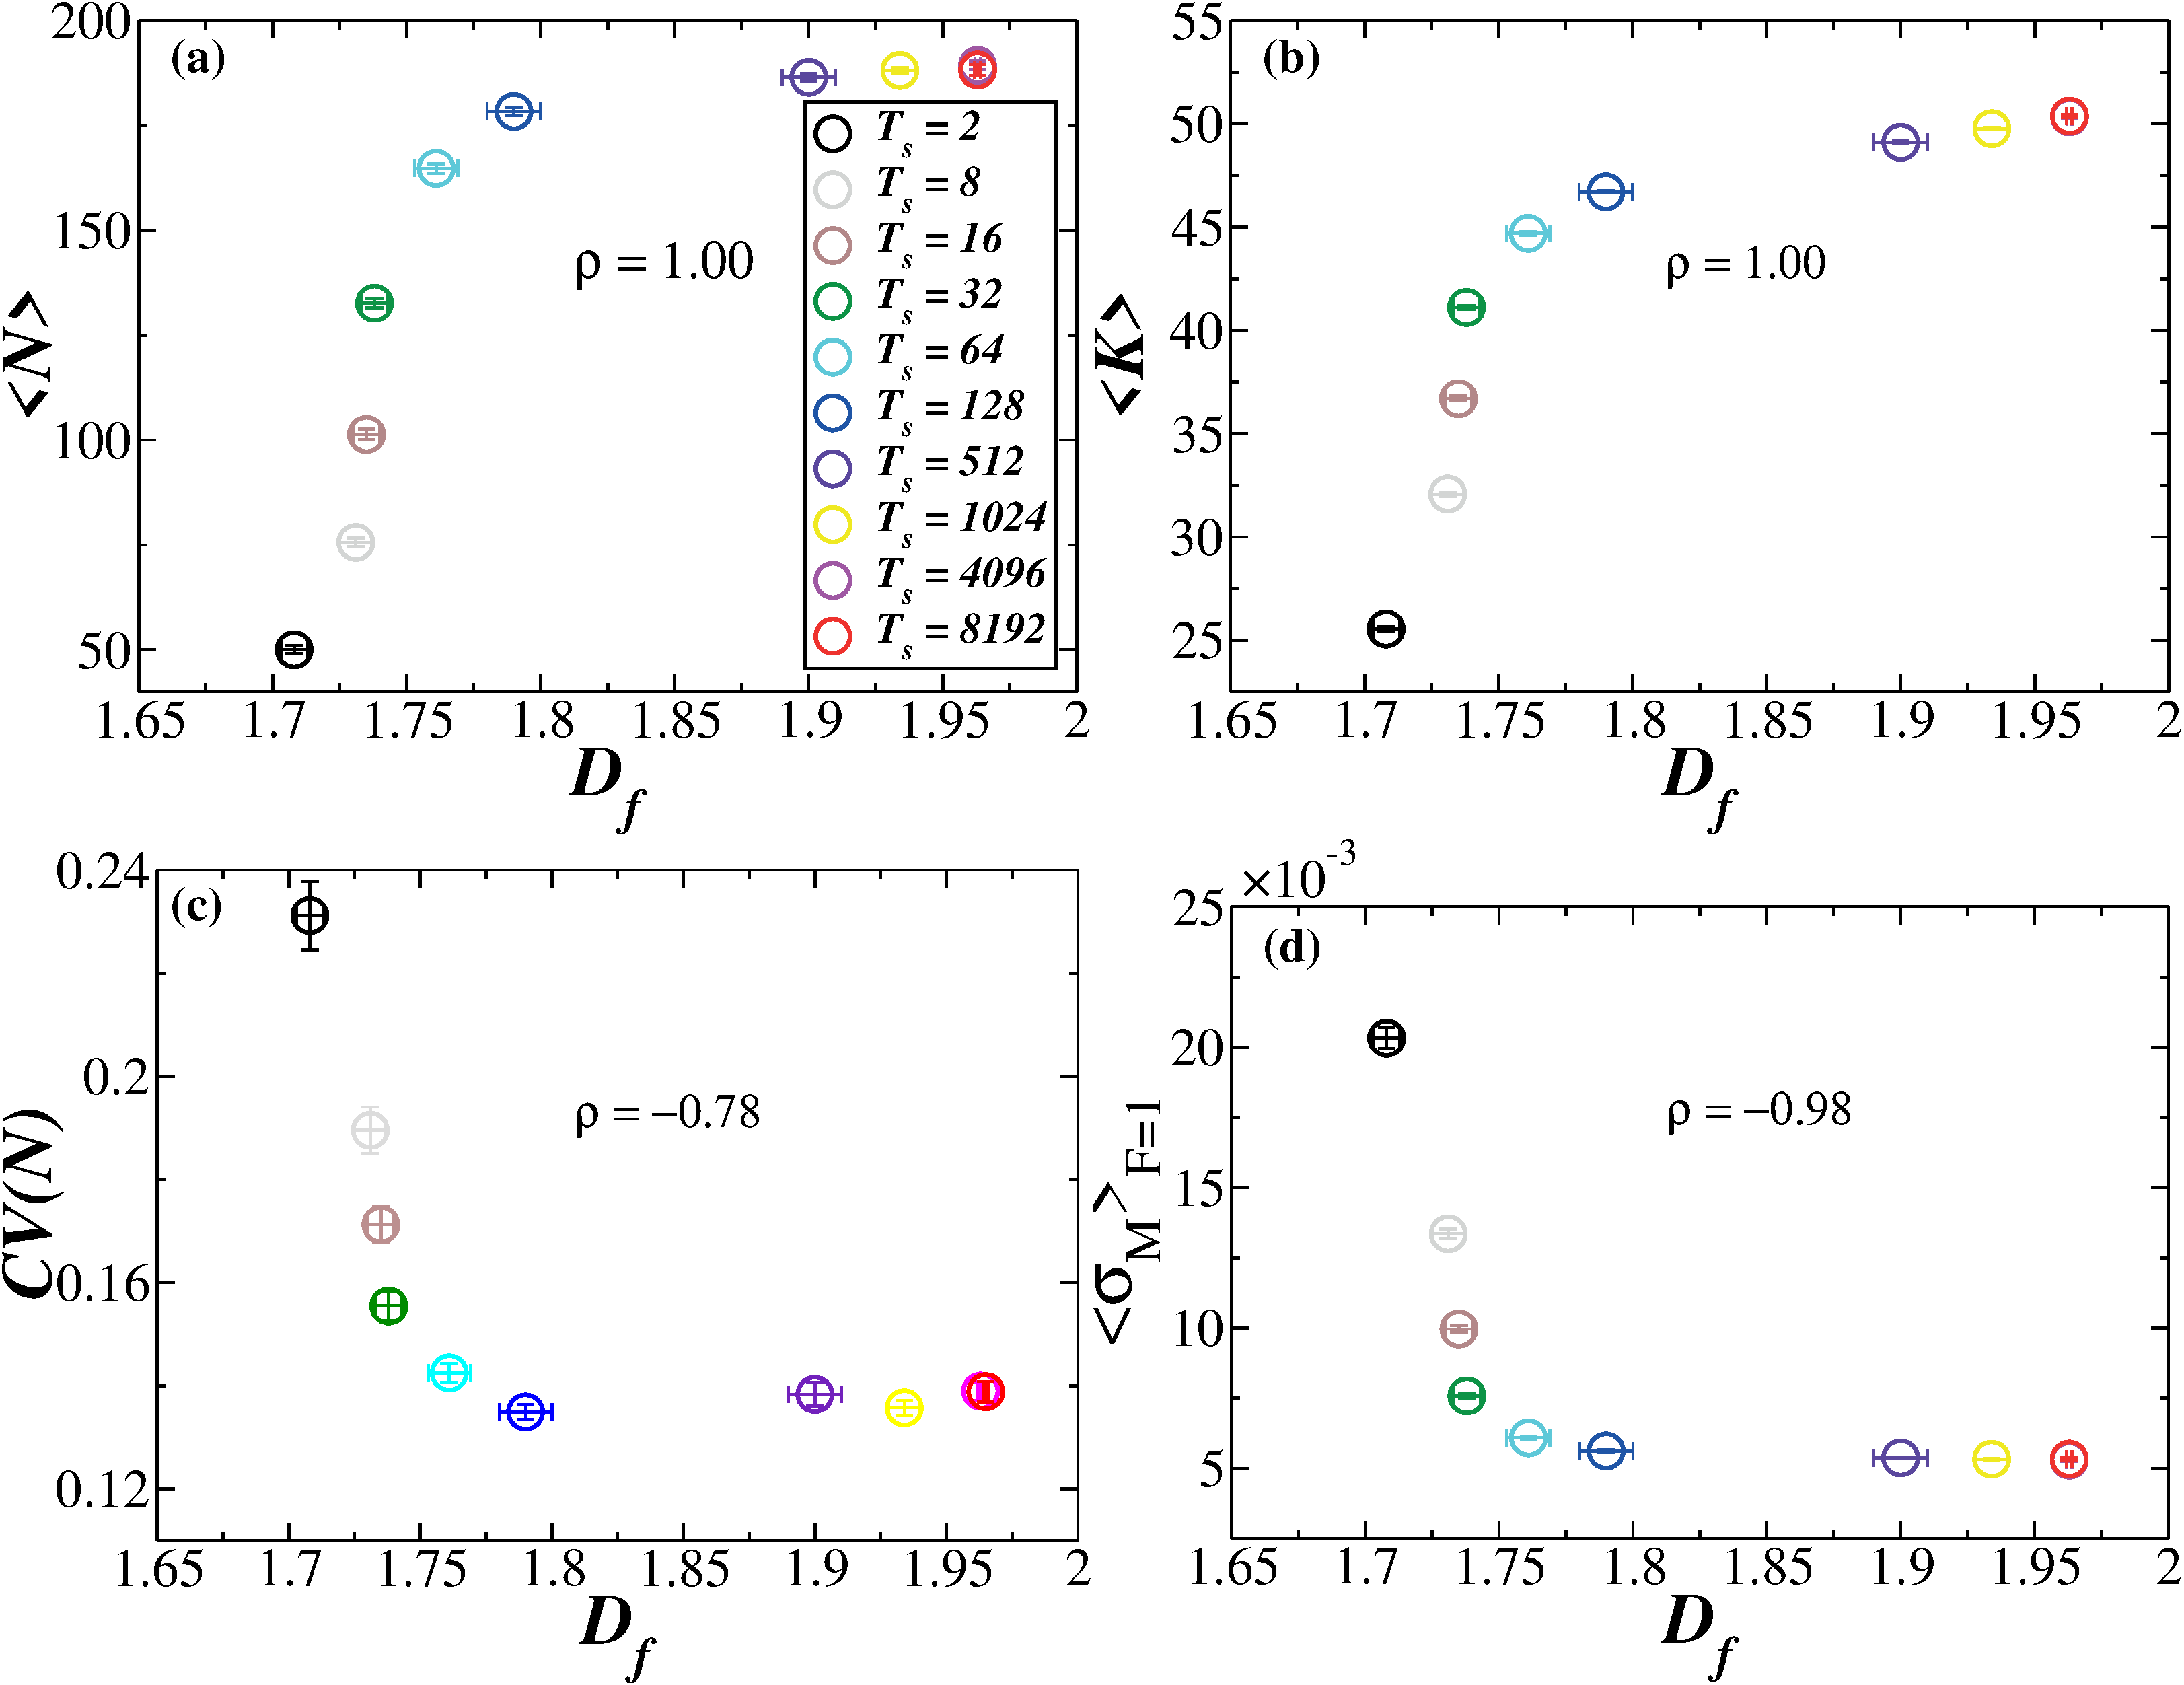
\includegraphics[width=\textwidth]{figure_4.pdf}
  \caption{Relationship between the cross-sectional fractal dimension \(D_f\)
  and structural descriptors of the three-dimensional load-bearing backbone:
  (a) mean load-bearing area \(\langle N\rangle\); (b) mean molecular
  coordination \(\langle K\rangle\); (c) axial coefficient of variation of
  the load-bearing area, \(\mathrm{CV}(N)\); and (d) mean molecular stress
  exposure at unit force, \(\langle\sigma_M\rangle_{F=1}\). Each point
  represents the ensemble average for one value of \(T_s\). Horizontal error
  bars are the standard errors of the mass--radius fits used to estimate
  \(D_f\), and vertical error bars are standard errors of the mean across
  fibrils. The reported \(\rho\) values are Spearman correlations across the
  ten \(T_s\) conditions. This figure is reproduced from Fig.~7 of the revised
  manuscript.}
  \label{fig:response-df-backbone}
\end{figure}

Taken together, these results provide direct numerical validation that \(D_f\)
captures structural changes relevant to axial load bearing: increasing \(D_f\)
corresponds to larger, better-coordinated, and more axially uniform
load-bearing backbones, with lower mean stress exposure for the same applied
force. Within its stated scope, which is the comparison of fibril ensembles
generated at different \(T_s\), \(D_f\) therefore provides a compact and
quantitatively supported proxy for mechanically relevant transverse
compactness. We have revised the manuscript to make this interpretation and
its scope explicit.

\pointseparator

\subsection*{Point 5 (R1-5): Empirical structural-mechanical connection}

\refereelabel
\begin{refereecomment}
The key result of the paper, that \(D_f\) and \(\gamma\) saturate together at
\(T_s\geq512\), is presented as if it were a derived causal relationship. In
fact, it is a numerical correlation observed in simulation. No theoretical
framework is provided that connects the fractal dimension of the fibril
cross-section to the avalanche exponent of the fracture process. The statement
that ``the fibril's fractal dimension serves as a quantitative bridge between
structural compactness and failure statistics'' in the Conclusion overstates
what has been demonstrated. The authors should reframe this as an empirical
observation and discuss what theoretical framework might, in the future,
explain such a connection.
\end{refereecomment}

\responselabel
We thank the Referee and agree that the coincident evolution of \(D_f\) and the
avalanche statistics does not establish a derived or causal relationship. Both
quantities change as the common control parameter \(T_s\) modifies fibril
architecture, but this common dependence alone does not demonstrate that the
cross-sectional fractal dimension determines the avalanche-size distribution.
We have therefore removed the statement that \(D_f\) provides a
``quantitative bridge'' between structure and failure statistics.

The revised manuscript now distinguishes two levels of evidence. First, the
analysis summarized in Fig.~\ref{fig:response-df-backbone} establishes that
\(D_f\) is strongly associated with mechanically relevant properties of the
three-dimensional backbone, including its load-bearing area, molecular
coordination, axial heterogeneity, and molecular stress exposure. Second, the
avalanche statistics also vary with \(T_s\). The coexistence of these trends is
reported only as an empirical association within the present model; it is not
used to infer causality, a universal scaling relation, or a particular
stress-redistribution mechanism.

A predictive theoretical connection would require an explicit framework that
propagates changes in three-dimensional network topology and cross-sectional
load-bearing heterogeneity into stress redistribution and cascade statistics.
Such a development would likely require elastic or viscoelastic force
transmission, together with sensitivity analyses of the molecular geometry and
rupture rule. These extensions lie beyond the present coarse-grained model and
are identified as directions for future work. The Results and Conclusion have
been revised to state this scope explicitly.

\pointseparator

\subsection*{Point 6 (R1-6): Molecular aspect ratio}

\refereelabel
\begin{refereecomment}
The aspect ratio of model molecules (18:1) differs substantially from that of
real collagen molecules (\(\approx 200{:}1\)). The impact of this
simplification on the fractal dimension and packing geometry should be
acknowledged.
\end{refereecomment}

\responselabel
We thank the Referee and agree that the reduced molecular aspect ratio is an
important limitation. Our model adopts the \(18\times1\times1\) lattice-rod
representation used by Parkinson et al. (1997), corresponding to an aspect
ratio of \(18{:}1\). This provides continuity with the original collagen
aggregation and fracture framework, but remains a substantial geometric
simplification relative to the approximately \(200{:}1\) aspect ratio of real
collagen molecules.

The reduced aspect ratio may affect molecular overlaps and local coordination,
packing and void geometry, and consequently the measured cross-sectional
fractal dimension \(D_f\) and the mechanically relevant quantities \(N(i)\),
\(\mathrm{CV}(N)\), and \(K\). Since \(N(i)\) and \(K\) determine molecular
stress exposure and removal probability in the rupture model, quantitative
damage curves, rupture resistance, and avalanche statistics may also depend on
the assumed aspect ratio.

Although the same aspect ratio is used for all \(T_s\), providing a consistent
geometry for comparisons within the model, this does not establish that the
numerical values or observed trends are independent of the aspect-ratio
approximation. Because an aspect-ratio sensitivity analysis was not performed,
the results should be interpreted as trends within the present coarse-grained
model rather than as quantitative predictions for real collagen fibrils. We
have revised the Methods to cite the origin of the \(18{:}1\) representation
and expanded the limitations section to state its possible structural and
mechanical consequences.

\pointseparator

\subsection*{Point 7 (R1-7): Phenomenological damage function}

\refereelabel
\begin{refereecomment}
The phenomenological function \(f(F)\) in Eq.~(5) is purely empirical. Its
form is not derived from the model and the physical interpretation of the
parameters \(\alpha\) and \(\beta\), while discussed qualitatively, would
benefit from more precise justification.
\end{refereecomment}

\responselabel
We thank the Referee for this observation. We agree that Eq.~(5) is a
phenomenological representation of the simulated damage curves rather than a
constitutive law derived from the microscopic removal rule. We have revised the
manuscript to clarify the functional roles of \(\alpha\) and \(\beta\) and to
relate their trends qualitatively to the structural quantities entering the
rupture model.

The \(F^{\alpha}\) contribution describes the gradual accumulation of damage at
low and intermediate forces. Mathematically, \(\alpha\) is the logarithmic slope
of this contribution and therefore controls its nonlinear sensitivity to
force. Its decrease with increasing \(T_s\) is consistent with the larger
load-bearing areas and greater molecular coordination of more compact fibrils.
A larger \(N(i)\) reduces the stress increase produced by a given force
increment through \(\sigma(i)=F/N(i)\), while a larger \(K\) decreases the
molecular removal probability. These structural changes buffer gradual damage
accumulation, producing the weaker force dependence represented by smaller
values of \(\alpha\). Because \(\alpha\) describes the cumulative damage curve,
it is treated as an effective force-sensitivity exponent.

The exponential contribution describes the rapid amplification of damage at
larger forces. As molecules are removed, \(N(i)\) decreases in the affected
cross-sections and the coordination number \(K\) is reduced for neighboring
molecules. The resulting increase in molecular stress and decrease in local
resistance create a positive feedback for subsequent removal. The parameter
\(\beta\) controls the force sensitivity of this late-stage amplification,
while \(1/\beta\) provides its characteristic force scale within the
dimensionless model. Its decrease with \(T_s\) is therefore consistent with the
delayed amplification observed in more compact and better-connected fibrils.

The revised discussion presents the two terms as complementary descriptions of
gradual damage accumulation and its subsequent amplification, rather than as
independent microscopic mechanisms. Their common approach to a plateau for
\(T_s\geq512\) also parallels the saturation of the structural characteristics
of the load-bearing backbone.

\pointseparator

\clearpage
\section*{\LARGE Response to Referee 2}

\subsection*{Point 1 (R2-1): Loading protocol and stability of the system}

\refereelabel
\begin{refereecomment}
My main concern is the loading protocol. Equation (4) defines the probability
of failure. As long as fibers carry load, this probability remains finite.
This seems to imply that, at any finite load, the bundle would fail after a
finite time, with a characteristic time depending on the load level. The
authors state that during a sweep through the system, each fiber is given a
chance to fail according to Eq.~(4), and if no failure occurs, the external
load is increased. This procedure appears somewhat artificial. If I understand
the model correctly, the bundle is not fully relaxed after a sweep: failure
could continue in a subsequent sweep at the same load level. Moreover, fiber
removal increases (\(\sigma_M\)) and decreases (\(K\)), both of which increase
the rupture probability (\(P_R\)). Thus, the system does not seem to be in a
stable state when the external load is further increased. The authors should
clarify this point in the manuscript.
\end{refereecomment}

\responselabel
We thank the Referee for pointing out that the meaning of a no-removal sweep
was insufficiently explained. Our rupture model does not introduce physical
time, a dwell time at fixed load, or a thermally activated failure rate.
Accordingly, \(P_R\) is a dimensionless removal probability evaluated during
a discrete damage-update sweep, not a continuous-time hazard rate.

The loading and stopping rule follows the procedure introduced by Parkinson et
al. (1997). At a prescribed force \(F\), every molecule in the load-bearing
backbone is assessed once. If removals occur, the backbone is reassessed and
another damage sweep is performed at the same force. The force is increased by
\(\Delta F=0.5\) only after a complete sweep produces no new removal event, as
specified in the original model.

We agree that a no-removal sweep does not establish an absorbing stochastic
equilibrium. Because \(P_R\) can remain nonzero, another independent assessment
of the same unchanged configuration could produce additional removals. The
first no-removal sweep is instead the operational stopping criterion of this
discrete, progressively stepped loading protocol, separating the damage
response assigned to the current force from that produced after the next force
increment.

Consequently, the model characterizes failure under stepped loading and is not
intended to describe creep, fatigue, delayed rupture, or lifetime under a force
held constant for a physical duration. We have revised the Methods to make this
interpretation and its limitations explicit.

\pointseparator

\subsection*{Point 2 (R2-2): Localized versus equal load sharing}

\refereelabel
\begin{refereecomment}
The authors discuss localized and more equal load-sharing regimes in their
interpretation. However, in the simulations, load sharing appears to be
determined by Eqs.~(2) and (3), which seem to impose equal load sharing within
a cross section. If I understand correctly, information about the local
structure enters only through \(K\) in the rupture probability. The authors
should discuss more clearly in what precise sense the model realizes localized
or equal-load-sharing behavior.
\end{refereecomment}

\responselabel
We thank the Referee for identifying this ambiguity. We agree that the original
interpretation invited the conclusion that our model realizes a crossover
between localized and equal load sharing. In particular, we compared the
fitted values of \(\gamma\) with exponents from fiber-bundle theory and
described their variation with \(T_s\) as evidence of increasingly global load
sharing. This interpretation was not supported by the stress-redistribution
rule implemented in the model. Numerical proximity between a fitted slope and
a theoretical fiber-bundle exponent is not sufficient to establish a common
load-sharing mechanism or universality class.

Equation~(2) distributes the applied force uniformly among all load-bearing
molecular segments within each cross-section. When a molecule is removed,
\(N(i)\) decreases only in the cross-sections previously occupied by that
molecule, and the corresponding stress increase is shared uniformly among the
remaining segments within each affected cross-section. The model does not
contain a distance-dependent elastic kernel that preferentially transfers this
additional stress to the spatial neighbors of the removed molecule.

Local structure enters the rupture probability through the coordination number
\(K\). Removing a molecule reduces \(K\) for its nearest neighbors and therefore
lowers their resistance to subsequent removal. This produces spatially
heterogeneous rupture probabilities, but it does not constitute local load
sharing in the conventional fiber-bundle sense. Conversely, because \(N(i)\)
varies along the fibril and molecules span different sets of cross-sections,
the model is not a conventional equal-load-sharing fiber bundle governed by a
single globally shared stress.

We therefore describe the model as combining uniform load sharing within each
cross-section with local coordination-dependent resistance. We have removed
the interpretation of \(\gamma\) as evidence of a crossover between local and
global load sharing and no longer assign the model to either universality
class. Consistently with our response to R2-3, the primary statistical
observable is now the avalanche generated at a fixed force; spatially
connected clusters are retained only as a geometric damage diagnostic and do
not imply a local-load-sharing mechanism.

\pointseparator

\subsection*{Point 3 (R2-3): Definition of avalanches}

\refereelabel
\begin{refereecomment}
Since load sharing according to Eq.~(2) is global within a cross section, it
seems that no particular stress concentration can develop around failed
(removed) fibers in that cross section. If this interpretation is correct,
then the definition of avalanches may require further justification. If the
stress field is not localized around failed clusters, it is not obvious why
avalanches should be defined as steps in the growth of connected failed
clusters. An alternative, and possibly more natural, definition would be to
regard an avalanche as the set of fibers that fail between two consecutive
increments of the external force. The authors should make this aspect of the
work clearer.
\end{refereecomment}

\responselabel
We thank the Referee for this important observation. We agree that, because
the model does not contain a localized elastic stress-redistribution kernel,
the complete response generated at a fixed force is the more natural primary
avalanche observable. We have therefore adopted the definition suggested by
the Referee.

At each force level \(F\), all molecules removed during the repeated sweeps
performed before the next force increment are collected into one avalanche,
whose size is the total number of removed
molecules. Spatially disconnected removals at the same force belong to the
same event because they occur within the same response to the imposed drive.
This operational use of ``avalanche'' does not imply spatial connectivity or
system-spanning failure. The event that produces complete rupture is excluded from the
preterminal distribution analyzed statistically.

Spatially connected damage clusters remain a possible geometric diagnostic,
but they are no longer used as the primary avalanche-size observable in the
revised statistical analysis. We have revised the Methods, figures, and
terminology consistently with this force-step definition.

\pointseparator

\subsection*{Point 4 (R2-4): Power-law statistics and SOC}

\refereelabel
\begin{refereecomment}
The interpretation of power-law statistics in terms of self-organized
criticality should be treated with caution. In rupture processes the system is
gradually destroyed, and there is no healing mechanism by which failed fibers
could recover and carry load again. Therefore, the analogy with self-organized
critical systems may be problematic unless it is carefully qualified. I
suggest that the authors either provide a more detailed justification for this
interpretation or reformulate the discussion in more cautious terms.
\end{refereecomment}

\responselabel
We agree with the Referee that the externally driven and irreversible fracture
process should not be identified as Self-Organized Criticality. We have
removed that terminology and now describe the behavior as avalanche
dynamics during progressive damage in a driven disordered system. As detailed
in our response to R1-2, the revised unbinned maximum-likelihood analysis
supports a power-law tail with an exponential cutoff, rather than a pure
scale-free distribution. This formulation retains the statistically supported
algebraic tail while distinguishing it clearly from an SOC interpretation.

\clearpage
\section*{References cited in the responses}
\small
\begin{enumerate}
  \item Clauset, A., Shalizi, C. R., and Newman, M. E. J. (2009).
  Power-law distributions in empirical data. \textit{SIAM Review},
  \textbf{51}, 661--703.
  \href{https://doi.org/10.1137/070710111}{doi:10.1137/070710111}.

  \item Corral, A., Deluca, A., and Ferrer-i-Cancho, R. (2012).
  A practical recipe to fit discrete power-law distributions.
  \href{https://arxiv.org/abs/1209.1270}{arXiv:1209.1270}.

  \item Deluca, A., and Corral, A. (2013). Fitting and goodness-of-fit test of
  non-truncated and truncated power-law distributions.
  \textit{Acta Geophysica}, \textbf{61}, 1351--1394.
  \href{https://doi.org/10.2478/s11600-013-0154-9}{doi:10.2478/s11600-013-0154-9}.

  \item Gobeaux, F., Mosser, G., Anglo, A., Panine, P., Davidson, P.,
  Giraud-Guille, M.-M., and Belamie, E. (2008). Fibrillogenesis in dense
  collagen solutions: A physicochemical study. \textit{Journal of Molecular
  Biology}, \textbf{376}, 1509--1522.
  \href{https://doi.org/10.1016/j.jmb.2007.12.047}{doi:10.1016/j.jmb.2007.12.047}.

  \item Kadler, K. E., Hojima, Y., and Prockop, D. J. (1988). Assembly of type
  I collagen fibrils de novo. Between 37 and 41 degrees C the process is
  limited by micro-unfolding of monomers. \textit{Journal of Biological
  Chemistry}, \textbf{263}, 10517--10523.

  \item Kalbitzer, L., and Pompe, T. (2018). Fibril growth kinetics link
  buffer conditions and topology of 3D collagen I networks.
  \textit{Acta Biomaterialia}, \textbf{67}, 206--214.
  \href{https://doi.org/10.1016/j.actbio.2017.11.051}{doi:10.1016/j.actbio.2017.11.051}.

  \item Klaus, A., Yu, S., and Plenz, D. (2011). Statistical analyses support
  power law distributions found in neuronal avalanches. \textit{PLoS ONE},
  \textbf{6}, e19779.
  \href{https://doi.org/10.1371/journal.pone.0019779}{doi:10.1371/journal.pone.0019779}.

  \item Morozova, S., and Muthukumar, M. (2018). Electrostatic effects in
  collagen fibril formation. \textit{The Journal of Chemical Physics},
  \textbf{149}, 163333.
  \href{https://doi.org/10.1063/1.5036526}{doi:10.1063/1.5036526}.

  \item Parkinson, J., Brass, A., Canova, G., and Brechet, Y. (1997). The
  mechanical properties of simulated collagen fibrils. \textit{Journal of
  Biomechanics}, \textbf{30}, 549--554.

  \item Ponce-Alvarez, A., Jouary, A., Privat, M., Deco, G., and Sumbre, G.
  (2018). Whole-brain neuronal activity displays crackling noise dynamics.
  \textit{Neuron}, \textbf{100}, 1446--1459.
  \href{https://doi.org/10.1016/j.neuron.2018.10.045}{doi:10.1016/j.neuron.2018.10.045}.

  \item Schober, P., Boer, C., and Schwarte, L. A. (2018). Correlation
  coefficients: Appropriate use and interpretation. \textit{Anesthesia \&
  Analgesia}, \textbf{126}, 1763--1768.
  \href{https://doi.org/10.1213/ANE.0000000000002864}{doi:10.1213/ANE.0000000000002864}.

  \item Spearman, C. (1904). The proof and measurement of association between
  two things. \textit{The American Journal of Psychology}, \textbf{15},
  72--101. \href{https://doi.org/10.2307/1412159}{doi:10.2307/1412159}.

  \item Stauffer, D., and Aharony, A. (1994). \textit{Introduction to
  Percolation Theory}, 2nd ed. Taylor \& Francis, London.

  \item Yang, Y.-L., and Kaufman, L. J. (2009). Rheology and confocal
  reflectance microscopy as probes of mechanical properties and structure
  during collagen and collagen/hyaluronan self-assembly. \textit{Biophysical
  Journal}, \textbf{96}, 1566--1585.
  \href{https://doi.org/10.1016/j.bpj.2008.10.063}{doi:10.1016/j.bpj.2008.10.063}.

  \item Zapperi, S., Ray, P., Stanley, H. E., and Vespignani, A. (1999).
  Avalanches in breakdown and fracture processes. \textit{Physical Review E},
  \textbf{59}, 5049--5057.
  \href{https://doi.org/10.1103/PhysRevE.59.5049}{doi:10.1103/PhysRevE.59.5049}.
\end{enumerate}
\normalsize

\end{document}
